\section{Tests realisés pour valider le fonctionnement du TP}
\bframe{\footnotesize
\vspace{-0.2cm}

Les tests réalisés ont étés les suivants:\\
\begin{figure}[!h]
    \centering
    %\hspace{-0.45cm}    
    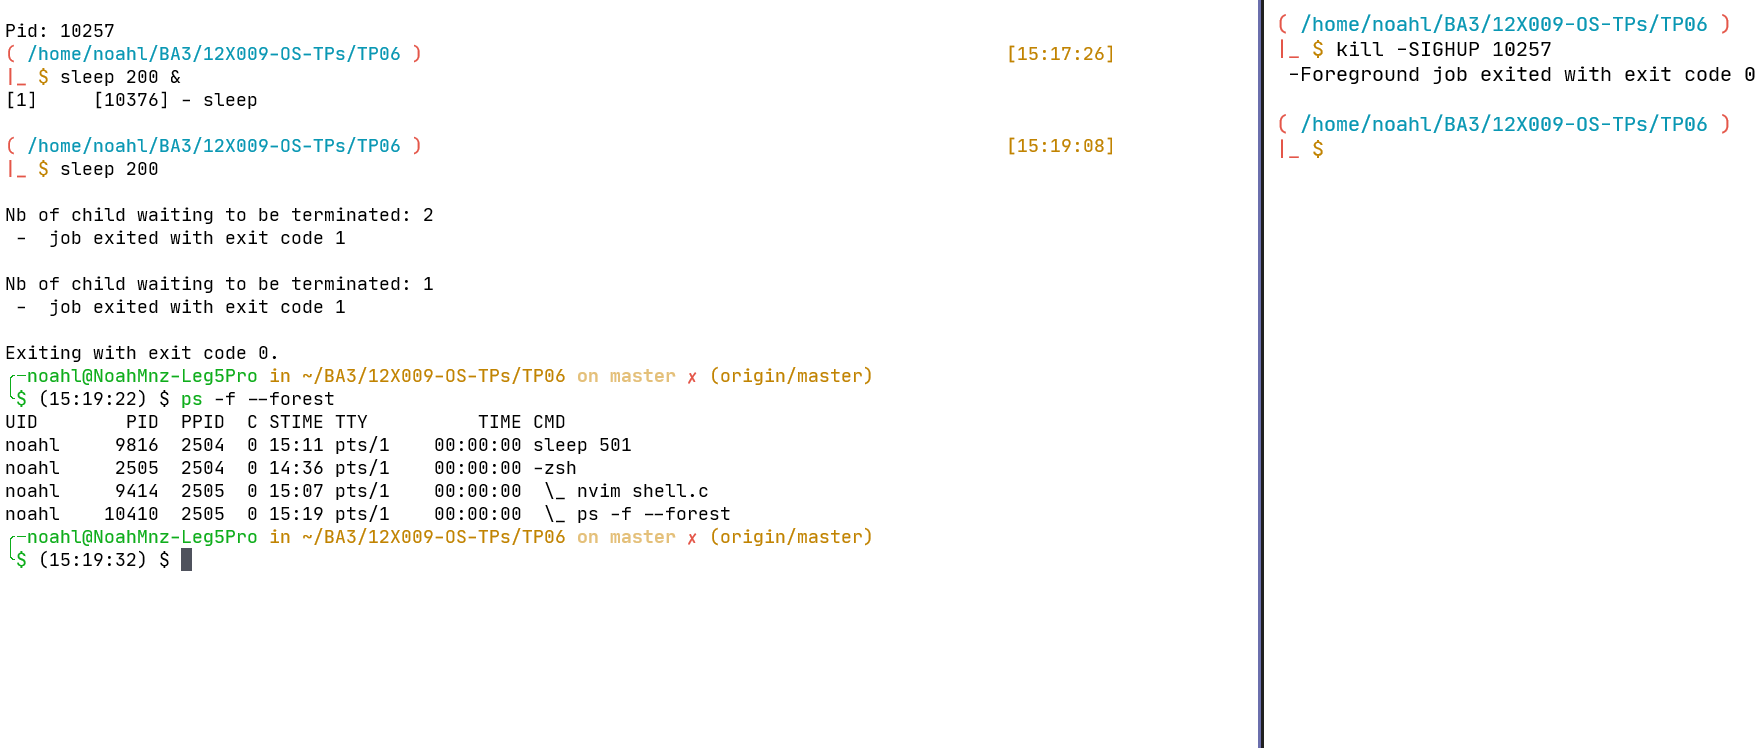
\includegraphics[width=12cm, height=6.9cm]{images/shell1.png}
    \caption{\footnotesize Gestion de Zombies/orphelin, background jobs + Gestion de signaux.\label{fig:shell1}}
\end{figure}
\unskip
}

\bframe{
\vspace{-0.2cm}
\begin{figure}[!h]
    %\centering
    %\hspace{-0.45cm}    
    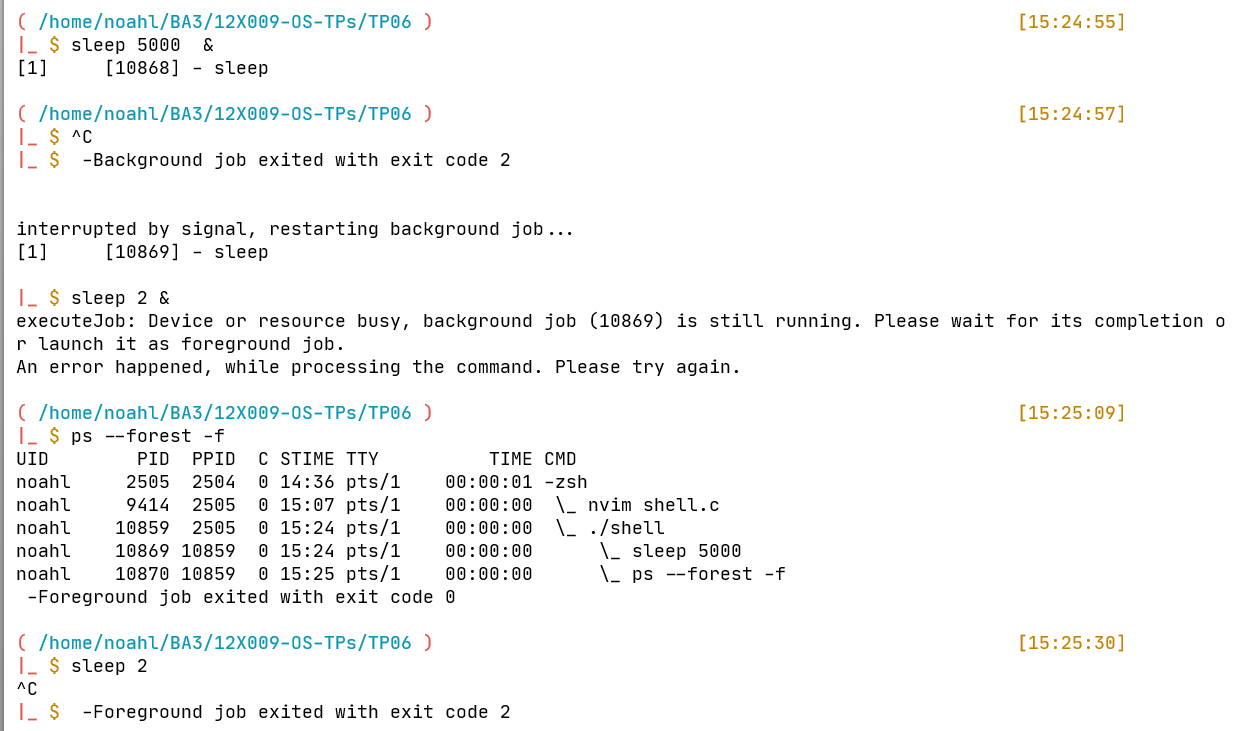
\includegraphics[width=10.5cm, height=7.2cm]{images/shell2.png}
    %\vspace{-0.20cm}

    \hspace{-1cm}
    \scriptsize \centering{Restart de processus en tâche de fond quand interrompu par signal \&
     1 seul BG job à la fois.}
    %\caption{\label{fig:shell2}}}
\end{figure}
\unskip
}

\begin{frame}
\vspace{-0.2cm}
\begin{figure}[H]
    \centering
    %\hspace{-0.45cm}    
    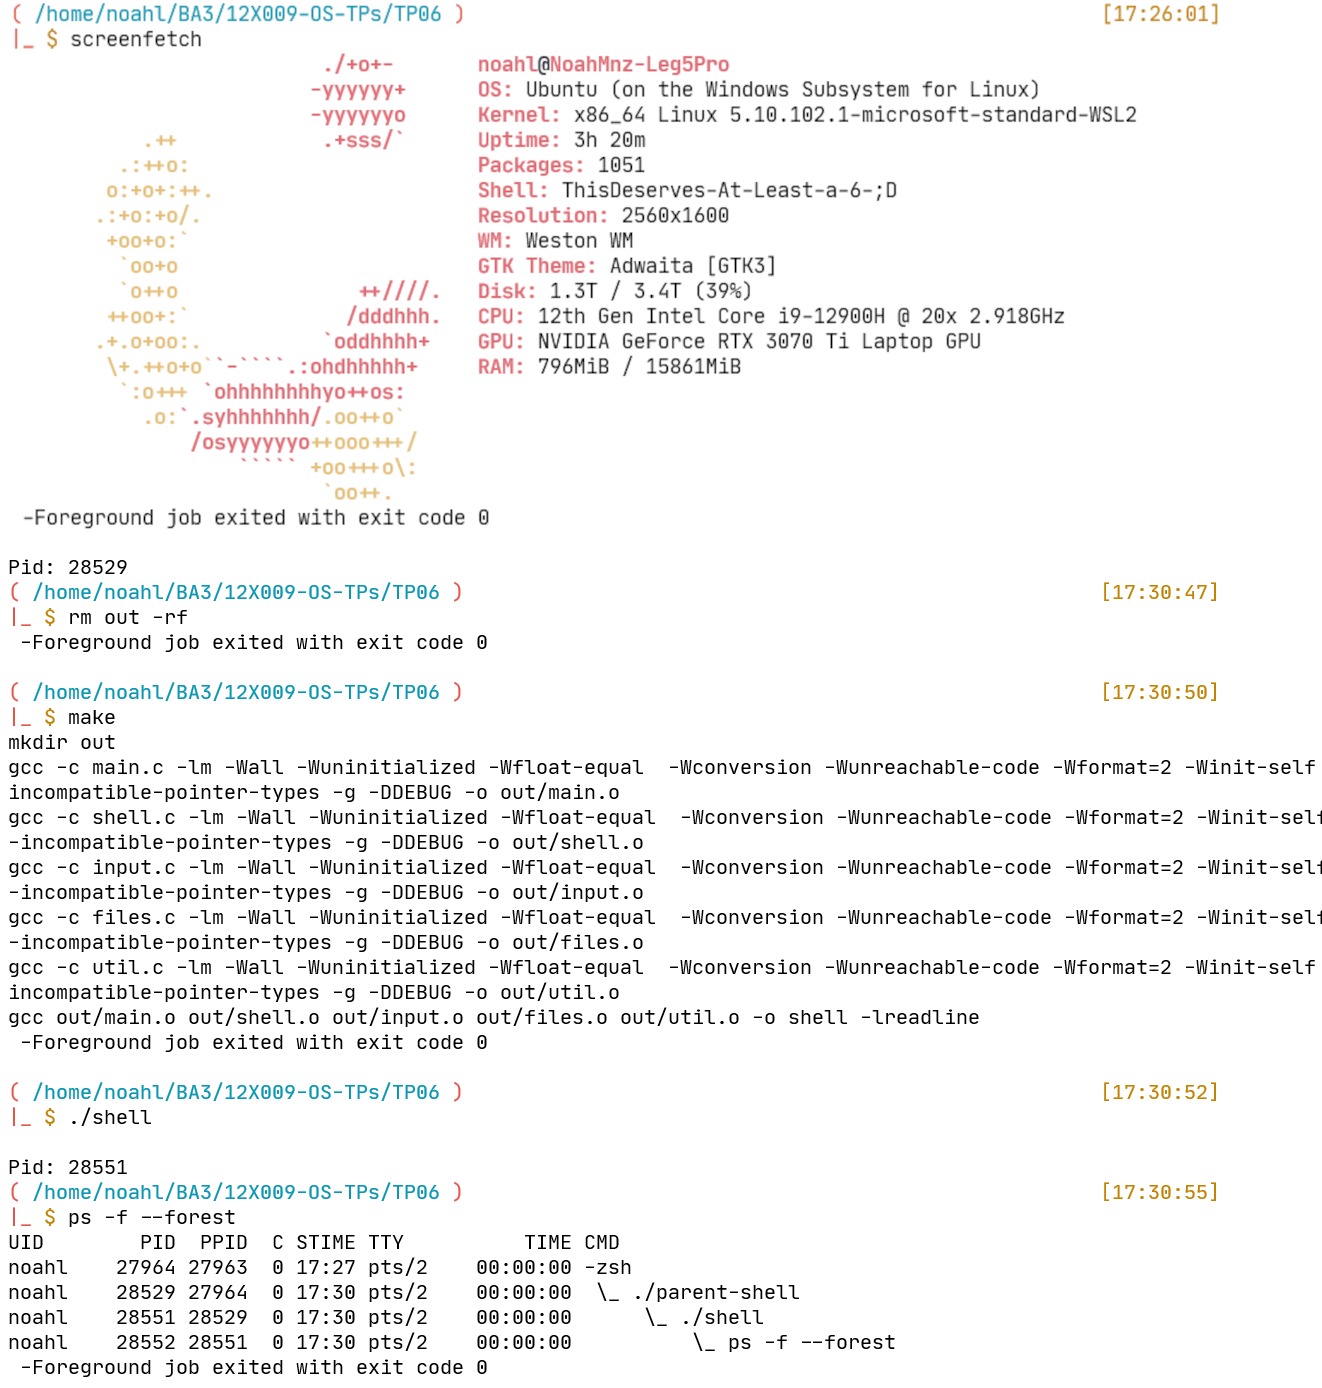
\includegraphics[height=0.75\columnwidth]{images/shell3.png}
    %\caption{\scriptsize Test de l'implémentation du TP05.\label{fig:shell3}}
\end{figure}
\unskip
\end{frame}

\bframe{
Où le but du dernier était de compiler le Shell dans le Shell puis le lancer toujours à partir du shell.
\vspace{0.5cm}

Aussi, pour tester SIGINT on a aussi lancé \code{tree /} (liste tous les fichiers depuis la racine formatté selon un arbre $\Rightarrow$ job très long qui nous le laisse le temps de le stopper) puis appuyé sur \code{ctrl+c} pour voir si ça arrêtait bien comme il le fallait.

\bigskip

\textbf{file descriptors}: Pour vérifier les redirections de \code{stdin} pour les background job, on a aussi utilisé les commandes \code{ lsof -a -p <pid>} 
et \code{ls /proc/<pid>/fd -la} (où \code{<pid>} est bien le pid du background job.)\\
La 2e est particulièment pratique vu qu'elle nous montre tout simplement quoi est ouvert et pointe vers quoi.
}